\documentclass[portrait,final,a0paper,fontscale=0.374]{baposter}

%% read in constants, custom functions and used packages

%%%%%%%%%%%%%%%%%%%%%%%%%%%%%%%%%%%%%%%%%%%%%%%%%%%%%%%%%%%%%%%%%%%%%%%% References paths
\usepackage[backend=biber, style=ieee, citestyle=ieee]{biblatex}
\addbibresource{refs.bib}
% font size
\AtBeginBibliography{\footnotesize}

%%%%%%%%%%%%%%%%%%%%%%%%%%%%%%%%%%%%%%%%%%%%%%%%%%%%%%%%%%%%%%%%%%%%%%%% Image paths
\usepackage{graphicx}
\graphicspath{{logos/}{figures/}}

%%%%%%%%%%%%%%%%%%%%%%%%%%%%%%%%%%%%%%%%%%%%%%%%%%%%%%%%%%%%%%%%%%%%%%%% Color Settings
\usepackage{xcolor}
\definecolor{iftucfont}{RGB}{74,130,70}
\definecolor{iftuccolor}{RGB}{143,168,92}
\definecolor{iftucbackground}{RGB}{241,244,234}

\definecolor{loop1}{HTML}{67AB9F}
\definecolor{loop2}{HTML}{FFB570}

\definecolor{direct}{HTML}{6C8EBF}
\definecolor{indirect}{HTML}{B85450}

\definecolor{training-set}{HTML}{EA6B66}
\setlength\bibitemsep{0.8\itemsep}

%%%%%%%%%%%%%%%%%%%%%%%%%%%%%%%%%%%%%%%%%%%%%%%%%%%%%%%%%%%%%%%%%%%%%%%% Font Settings
\usepackage[sfdefault, regular]{roboto}

%%%%%%%%%%%%%%%%%%%%%%%%%%%%%%%%%%%%%%%%%%%%%%%%%%%%%%%%%%%%%%%%%%%%%%%% Multicol Settings
\usepackage{multirow}
\usepackage{multicol}
\setlength{\columnsep}{1.5em}
\setlength{\columnseprule}{0mm}

%% Row Settings
\usepackage{setspace}% for \onehalfspacing
\usepackage{parskip}

%% Control layout of itemize, enumerate, description
\usepackage{enumitem}

% page borders and header height
\usepackage{geometry}
\geometry{
	left=35pt,
	right=5pt,
	top=10pt
}

\newcommand{\compresslist}{% Define a command to reduce spacing within itemize/enumerate environments, e.g. \begin{itemize}\compresslist
			\setlength{\itemsep}{1pt}
			\setlength{\parskip}{0pt}
			\setlength{\parsep}{0pt}
		}
	
\newcommand{\compressbib}{%
		\setlength{\itemsep}{0pt}
		\setlength{\parskip}{0pt}
		\setlength{\parsep}{0pt}
	}
	
%%%%%%%%%%%%%%%%%%%%%%%%%%%%%%%%%%%%%%%%%%%%%%%%%%%%%%%%%%%%%%%%%%%%%%%% Table and figure settings
\usepackage{float, booktabs, array, ragged2e}

% Adjust row width in tables 
\renewcommand{\arraystretch}{1.1}

% for awesome plots and tables from files like .csv
\usepackage{pgfplots}
\usepackage{pgfplotstable}

\usepackage{algorithm}
\usepackage{algpseudocode}

\usepackage{listings}
\lstset{
	basicstyle=\footnotesize\ttfamily,
	numbers=left,
	numberstyle=\tiny,
	stepnumber=1,
	numbersep=5pt,
	backgroundcolor=\color{white},
	showspaces=false,
	showstringspaces=false,
	showtabs=false,
	tabsize=2,
	captionpos=b,
	breaklines=true,
	breakatwhitespace=true,
	breakautoindent=true,
	linewidth=\columnwidth
}

% Graphics package-alike macros for “general” boxes. Like resizing figures and aligning minipages
\usepackage{adjustbox}

\usepackage[
font=footnotesize,
labelfont=bf,
%labelfont=sc, %Kapitälchen, passt nicht wg. nicht-osf Ziffern
%%%%labelfont=it, %italics, 
%%%labelfont=sl, %slanted,
hypcap=true,
format=hang,
%margin={2cm,2cm}
width=0.8\linewidth
]{caption}

%%%%%%%%%%%%%%%%%%%%%%%%%%%%%%%%%%%%%%%%%%%%%%%%%%%%%%%%%%%%%%%%%%%%%%%% Other packages
% to help with long equations
\usepackage{amsmath}

% for todo notes
\usepackage{todonotes} 

% for comment blocks
\usepackage{verbatim}

% link URLs
\usepackage{url}

\usepackage{lipsum}


\begin{document}

\begin{poster}%
	% Poster Options
	{
		% Show grid to help with alignment
		grid=false,
		% Number of columns and column spacing
		columns=6,
		colspacing=1em,
		% Color style
		bgColorOne=white,
		borderColor=iftuccolor,
		headerColorOne=iftucbackground,
		headerFontColor=iftucfont,
		boxColorOne=white,
		% Format of textbox
		textborder=rounded,
		textfont=\small,
		% Format of text header
		eyecatcher=true,
		headerborder=closed,
		headerheight=0.1\textheight,
		%  textfont=\sc, An example of changing the text font
		headershape=rounded,
		headershade=plain,
		headerfont=\Large\bf, %Sans Serif
		% textfont={\setlength{\parindent}{1.5em}},
		boxshade=plain,
		%  background=shade-tb,
		background=plain,
		linewidth=2pt
	}
	% University logo
	{\includegraphics[height=6.5em]{tuckhseng_color}} 
	% Title
	{\bf\Large{Neurocomputational Modeling of Sensorimotor Integration via Cortico-Basal Ganglia-Thalamic Loops}\vspace{6pt}}
	% Authors
	{\normalsize Erik~Syniawa\textsuperscript{1} and Fred~Hamker\textsuperscript{1} \\ \vspace{0.8em}
	
	\small\textsuperscript{1} Professorship Artificial Intelligence, Department of Computer Science, \\ Chemnitz University of Technology, Chemnitz, Germany \\ \vspace{0.5em}
	\small Contact: fred.hamker@informatik.tu-chemnitz.de
	}
	% Department logo and other logos
	{	
		\begin{minipage}[r]{0.1\textwidth}
			
\includegraphics[height=7em]{active_self_logo_color}
		\end{minipage}
		\hfill
		\begin{minipage}[r]{0.1\textwidth}
			
\includegraphics[height=6.5em]{TUC_AI_color}
		\end{minipage}
		
	}

%%%%%%%%%%%%%%%%%%%%%%%%%%%%%%%%%%%%%%%%%%%%%%%%%%%%%%%%%%%%%%%%%%
% use height in headerbox to align multiple boxes 
% height= <size in percent of column height>, else [auto]%
\headerbox{Introduction}{name=infos,column=0,row=0, span=2, height=0.092}{
	\begin{adjustbox}{minipage=0.95\textwidth, margin=5pt, center}
		\justifying
		\textit{Sensorimotor integration} is crucial for early human development, yet its neural mechanisms are not fully understood.\\ Our study presents a neurocomputational model that explores the interplay between the cortex, basal ganglia, and thalamus in this process, with a focus on the centro median nuclei (CM) of the intralaminar nuclei (ILN) of the thalamus.\\
	\end{adjustbox}
}

\headerbox{Overview}{name=overview,column=2,row=0, span=4}{
	\begin{adjustbox}{minipage=0.95\textwidth, margin=5pt, center}
		\begin{minipage}[r]{0.28\textwidth}
			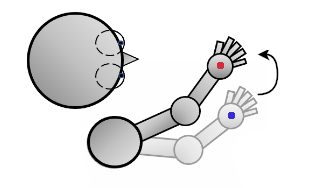
\includegraphics[width=0.9\linewidth]{movement_plan}
			\captionof{figure}{Current virtual robot setup.}
		\end{minipage}
		\hfill
		\begin{minipage}[r]{0.72\textwidth}
			\justifying
				\textbf{Task:}
				We implemented a virtual robot that can move from arbitrary \textcolor{blue}{starting position} to arbitrary \textcolor{red}{target position} in the plane (Figure 1)\\[3pt]
				\textbf{Training:}
				Through infant-like motor babbling, our network forms associations between the action (joint angle) and the outcome (position achieved)\parencite{baladronContributionBasalGanglia2023b}.The internal state (Joint angle of initial state) is projected via the CM into the CBGT loop, which ensures that action and outcome are learned under one internal state\\[3pt]
				\textbf{Features:}
				Shows how sensorimotor integration occurs through cortico-basal ganglia-thalamo-cortical loops with more dynamical role of the basal ganglia in both action selection and movement modulation \parencite{parkBasalGangliaCircuits2020}
		\end{minipage}
		\hfill
	\end{adjustbox}
}


\headerbox{Computational model}{name=model, column=0, below=infos, span=2, height=0.488}{
	\begin{adjustbox}{minipage=0.95\textwidth, margin=5pt, center}
		\begin{minipage}[t]{\textwidth}
			\centering
			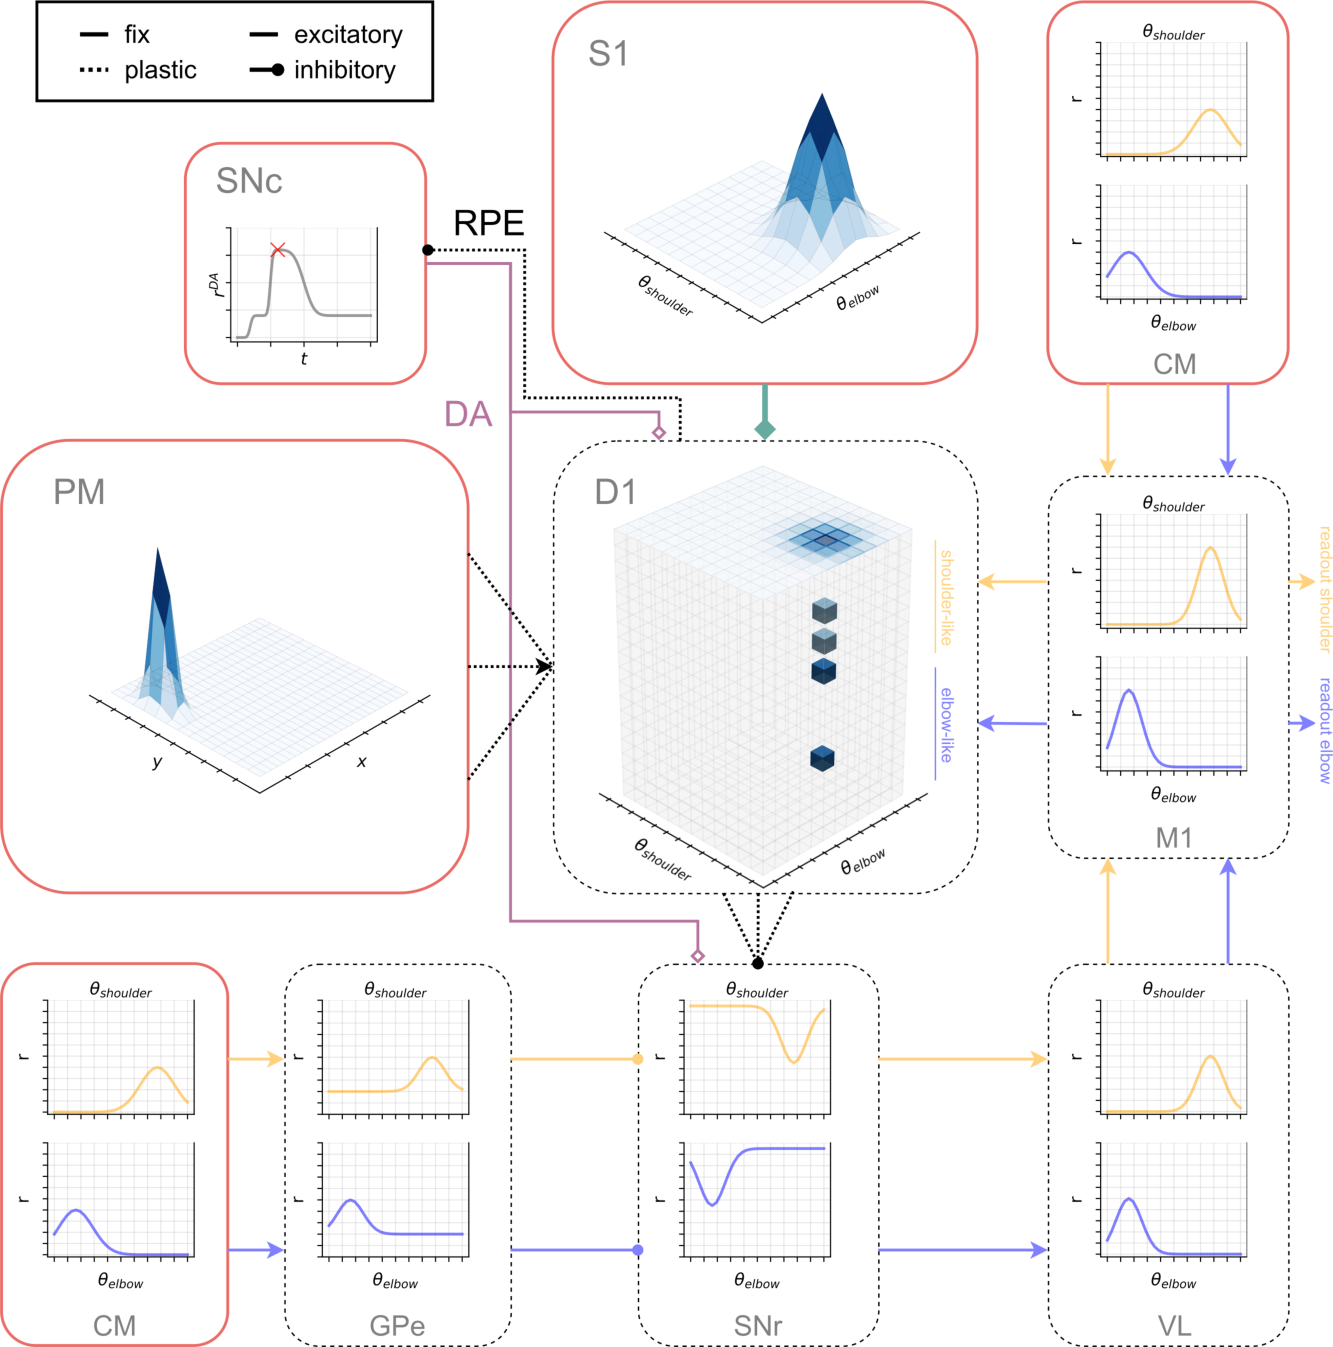
\includegraphics[width=\linewidth]{model_overview}
			\captionof{figure}{Overview of the model}
			\vspace{5pt}
		\end{minipage}
		\hfill
		\begin{minipage}[b]{\textwidth}
			\justifying
\textbf{\textcolor{training-set}{Input Populations}}:\\[4pt]
\footnotesize
\textbf{PM}: Encodes the target position in the reaching space. A 3-factor learning rule is used to establish connections to active D1 patches (see Model definitions).\\[2pt]
\textbf{S1}: Encodes current joint angles via gain fields. S1 sends projections that diverge to innervate multiple regions in the Striatum (D1 patches) \parencite{flahertyCorticostriatalTransformationsPrimate1991}\\[2pt]
\textbf{CM}: Centro median nuclei located in the intralaminar nuclei sends proprioceptive information of the target position into the M1. This connection is deactivated in the test phase.\\[10pt]
\small
\textbf{Recurrent Populations:}\\[4pt]
\footnotesize
\textbf{D1} (Striatum): Activity in S1 and M1 activates certain patches of D1 receptors in the striatum\\[2pt]
\textbf{SNr}: Pooling takes place from D1 $\rightarrow$ SNr. Active joint angle encodings in D1 inhibit corresponding neurons in SNr\\[2pt]
\textbf{VL}: Inactive SNr neurons disinhibit VL neurons\\[2pt]
\textbf{M1}: M1 encodes shoulder like and elbow like neurons via population code 
\parencite{pruszynskiPrimaryMotorCortex2011}, which map the joint angle to a specific coordinate. The weighted sum of the M1 activity is the angle of the corresponding joint\\[2pt]
\textbf{SNc}: Dopamine (DA) is released through movement \parencite{cheungLearningCriticallyDrives2023}, which makes the connections between PM $\rightarrow$ D1 plastic. Active D1 neurons inhibit DA release (\textit{RPE})

		\end{minipage}
	\end{adjustbox}
}


\headerbox{Model definitions}{name=definitions, column=2, below=overview, span=4}{
	\begin{adjustbox}{minipage=0.95\textwidth, margin=5pt, center}
		\begin{minipage}[r]{0.475\textwidth}
		The model is implemented in Python 3.12 with the neurosimulator ANNarchy 4.7.3 \parencite{vitayANNarchyCodeGeneration2015}. All neurons are rate-coded.\\
				
		\textbf{Neuron model:}\\
		$$
		\tau \frac{d r^{post}_j }{ dt } + r^{post}_j = \sum_{i \in exc}{w_{ij} \cdot r^{pre}_i} - \sum_{i \in inh}{w_{ij} \cdot r^{pre}_i} + baseline + \xi 
		$$
		$${mp}(t) = \begin{cases}\operatorname{logistic}{\left({r}(t) \right)}\qquad \text{if} \quad {r}(t) > 1.0\\ ({r}(t))^+ \qquad \text{otherwise.} \end{cases} \hspace{2em} \text{with:  } \xi \sim \mathcal{U}$$
		
		
		\textbf{Synaptic learning rule:}\\
		$$\tau_w \frac{d w_{ij} }{ dt } = m_{DA} \cdot C_{ij} - \alpha \left(r^{post}_j - \bar{r}^{post} - \gamma^{post}\right)^2$$
		\end{minipage}
		\hfill
		\begin{minipage}[r]{0.475\textwidth}
		\justifying
		$$m_{DA} = const \cdot \left(r^{DA} - baseline_{DA}\right) \hspace{1.5em} \tau_{\alpha} \frac{d \alpha_j }{ dt } + \alpha_j = (r^{post}_j - \Theta)$$
		\textit{Cortico-striatal} (PM $\rightarrow$ Striatum)
		$$ C_{ij} = \left(r^{pre}_j - \bar{r}^{pre} - \gamma^{pre}\right)^+ \left(r^{post}_j - \bar{r}^{post} - \gamma^{post}\right) $$	
		\textbf{Reward Prediction Error (RPE):}\\[5pt]
			When certain striatum neurons are repeatedly active, they inhibit the DA release ($r^{DA}$). 
			This prevents new associations from being learned by the same striatum neurons (\textit{novelty learning}).\\
			(Striatum $\rightarrow$ SNc)
			$$ \tau \frac{d w_{j}^{DA}}{dt} =  \left(r^{DA} - baseline_{DA}\right)^+ \left( r^{pre}_j - \bar{r}^{pre} - \gamma^{pre}\right)^+ $$
		\end{minipage}
	\end{adjustbox}
}

\headerbox{References}{name=refs, column=0, above=bottom, span=5}{
	\begin{adjustbox}{minipage=0.975\textwidth, margin=0pt, center}
		\compressbib{\printbibliography[heading=none]}
	\end{adjustbox}	
}

\headerbox{Results}{name=res, column=2, below=definitions, above=refs, span=4}{
	\begin{adjustbox}{minipage=0.95\textwidth, margin=5pt, center}
		\begin{minipage}[t]{0.475\textwidth}
			\textbf{Reaching:}\\[2pt]
			A random \textcolor{red}{target position} is activated in the PM. If the coordinate has been learnt, certain D1 neurons become active, which in turn encode the joint angle to the coordinate via the SNr activity in M1.\\[10pt]
		\begin{center}
			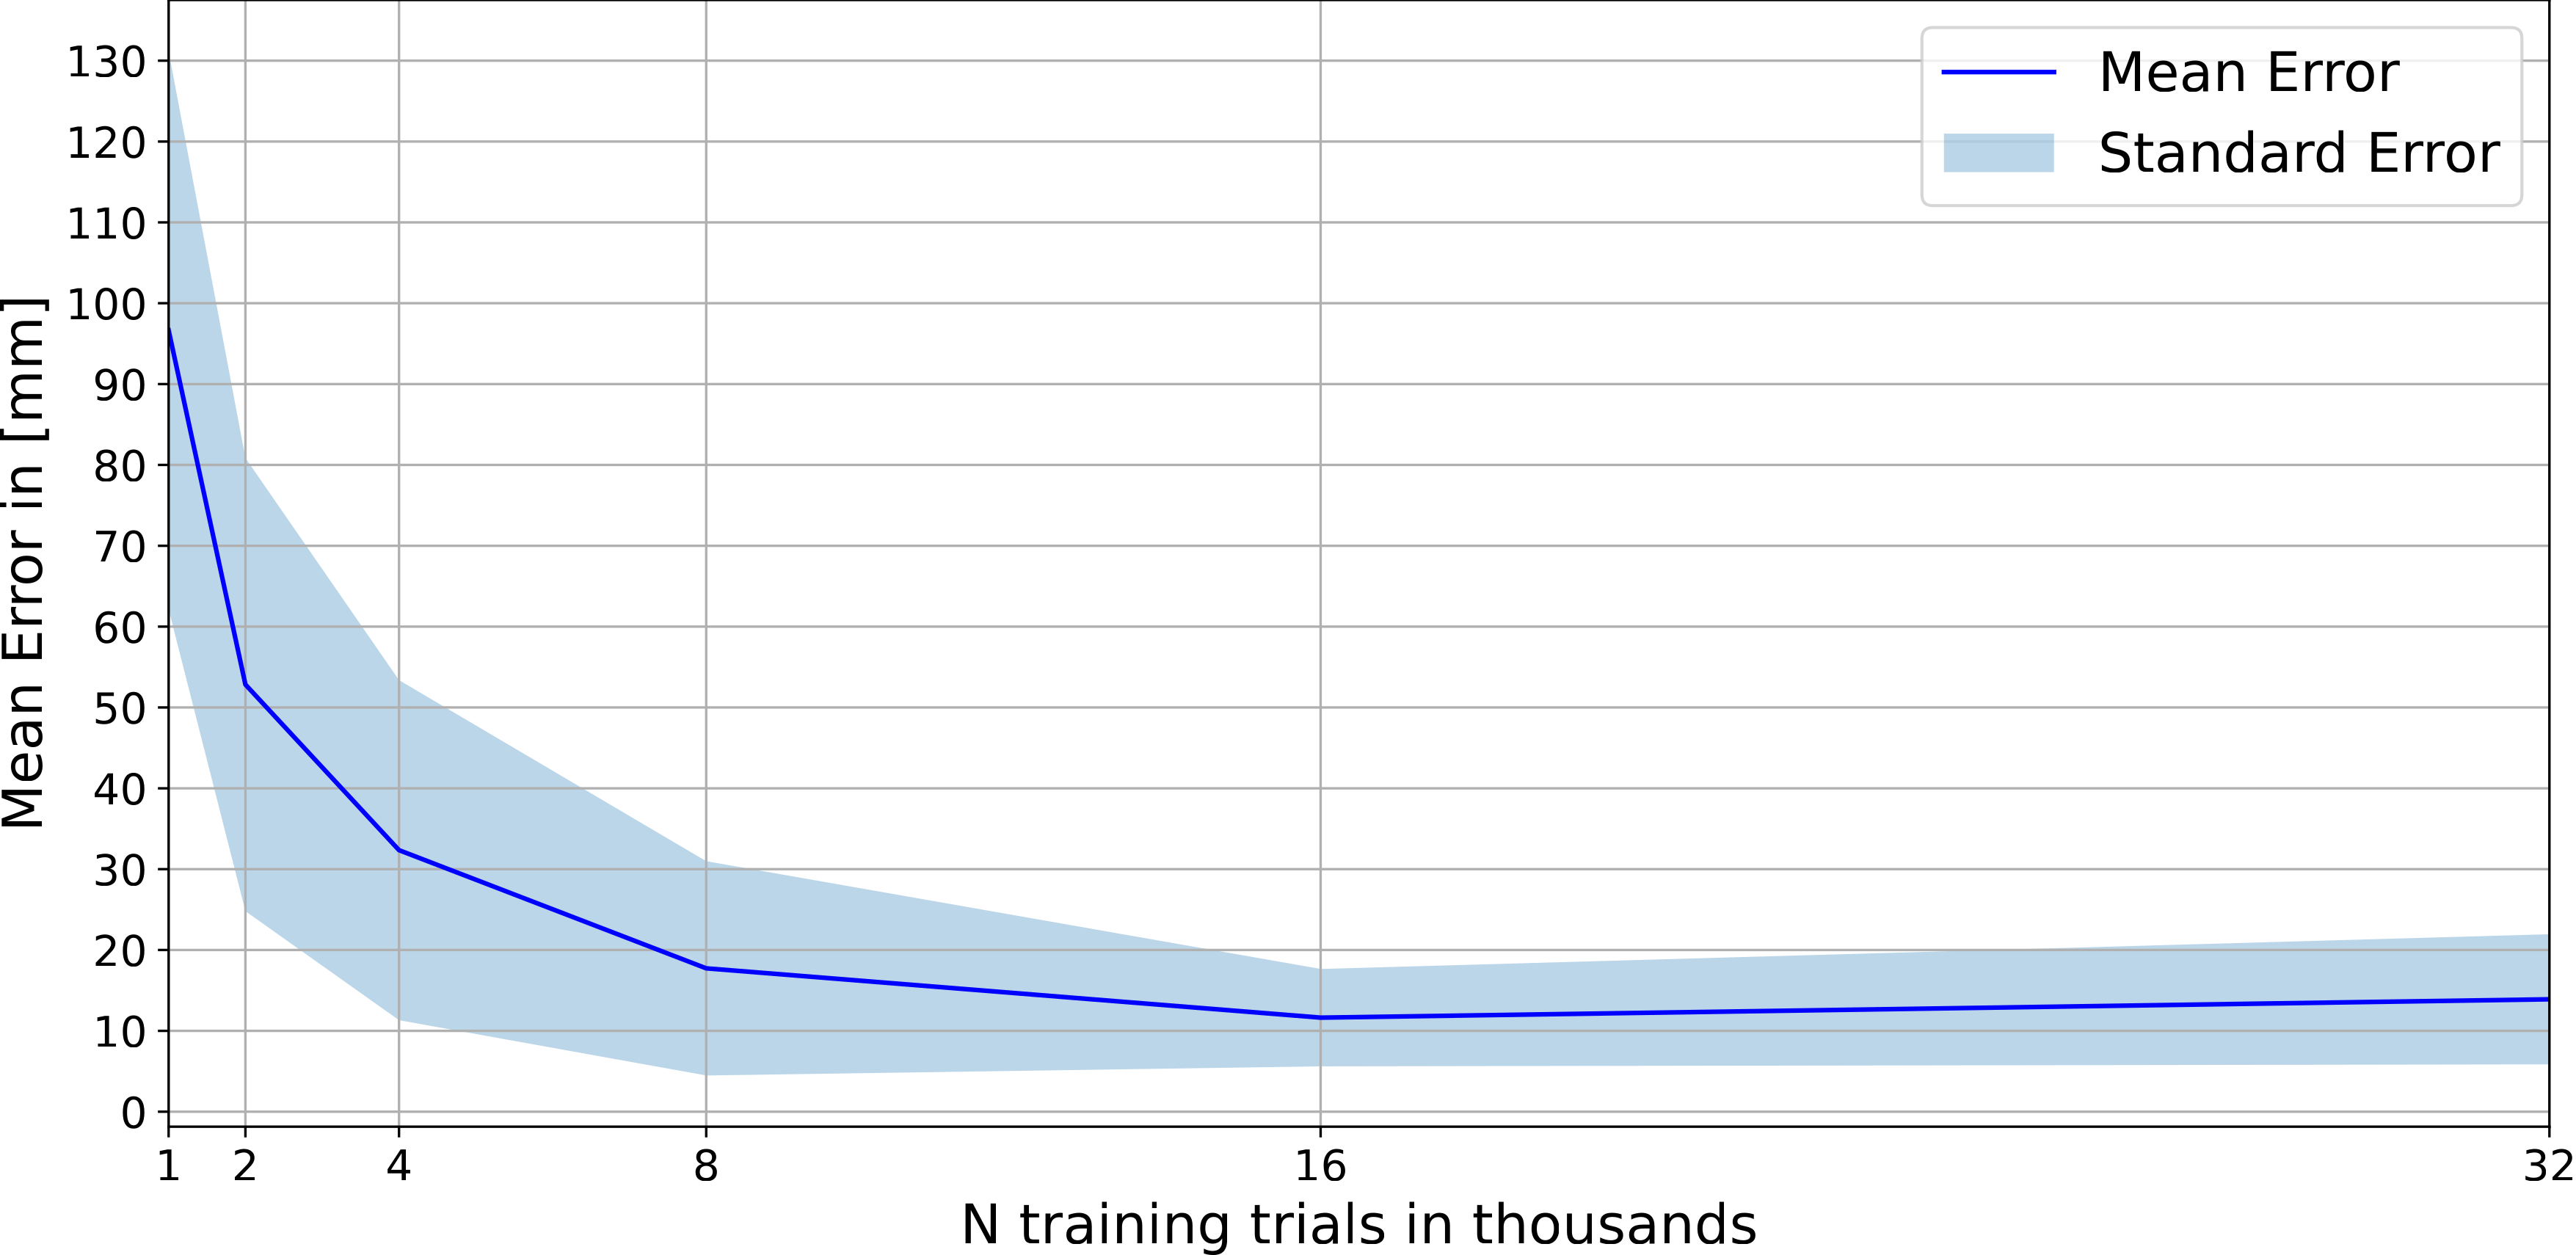
\includegraphics[width=\linewidth]{bg_error_plot}
			\captionof{figure}{Mean Error in the reaching task}
		\end{center}
		\end{minipage}
		\hfill
		\begin{minipage}[t]{0.475\textwidth}
			\textbf{Perturbation:}\\[2pt]
			A random \textcolor{red}{target position} is activated in the PM. As the activities build up, the joint angles in S1 are perturbed by a random amount by $\Delta \theta_{shoulder}$ and $\Delta \theta_{elbow}$. Both drawn from a Uniform Distribution $\mathcal{U}[-10^\circ, 10^\circ]$.\\
			\begin{center}
				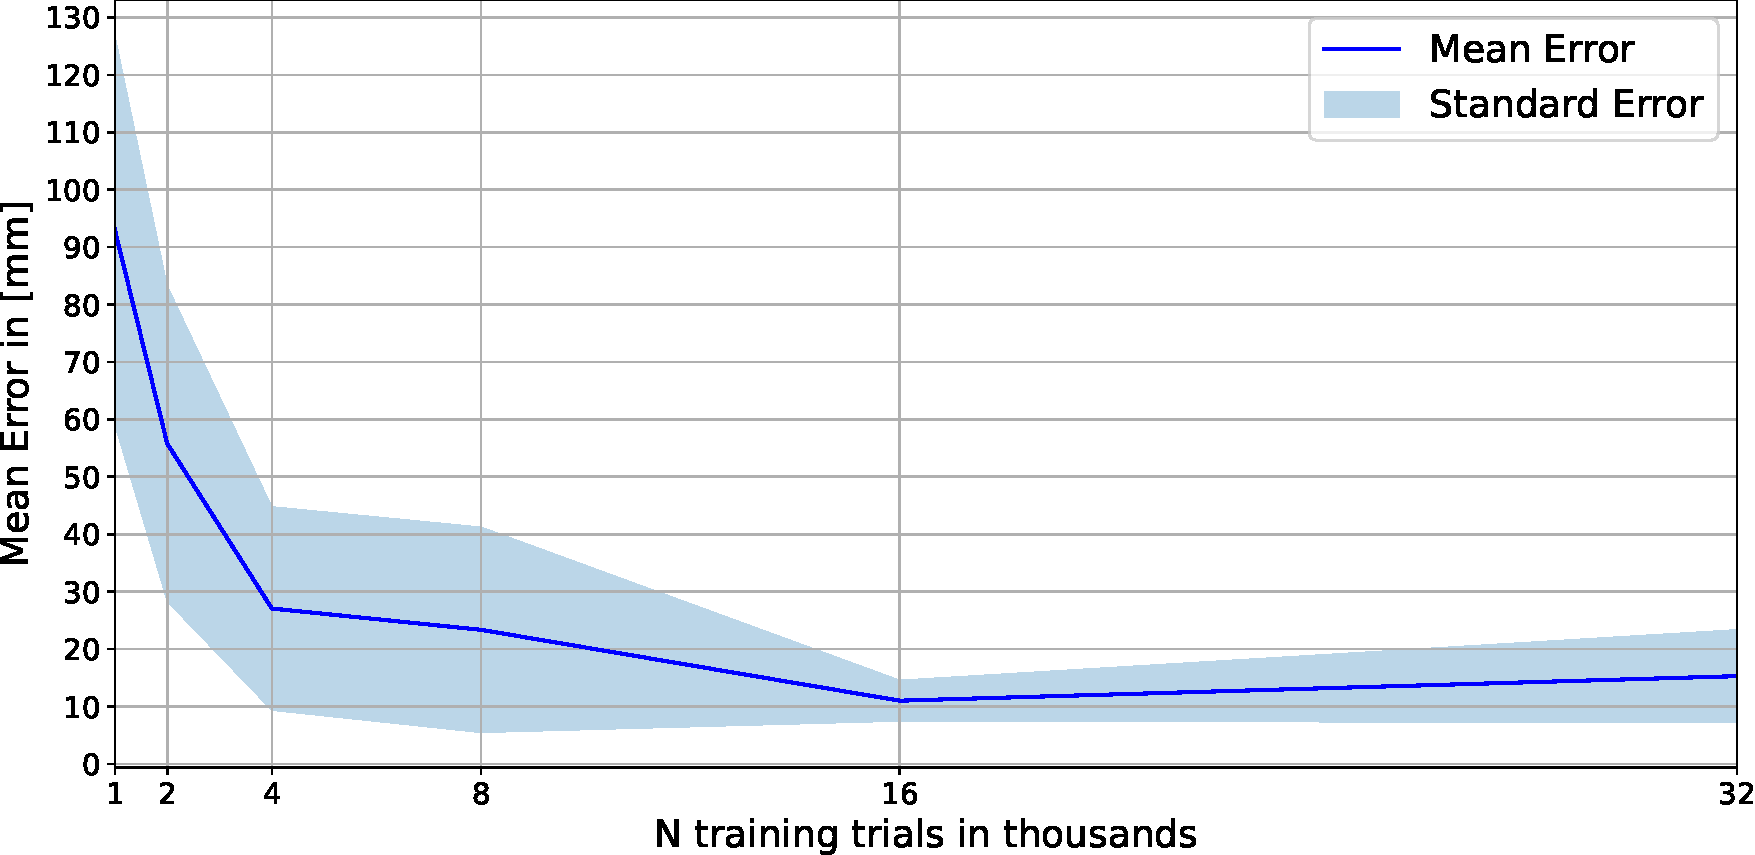
\includegraphics[width=\linewidth]{bg_error_plot_perturbation}
				\captionof{figure}{Mean Error in the perturbation task}
			\end{center}
		\end{minipage}
		\hfill
		\begin{minipage}[t]{0.25\textwidth}
			\vspace{8pt}
			\textbf{Modulation of the population code:}\\[2pt]
			A random target coordinate was learned. Figure 5 shows the population code of shoulder-like and elbow-like neurons under different scaling in D1. The activity of the D1 neurons has a direct influence on the norm of the population code \parencite{parkBasalGangliaCircuits2020}.\\
			\begin{center}
				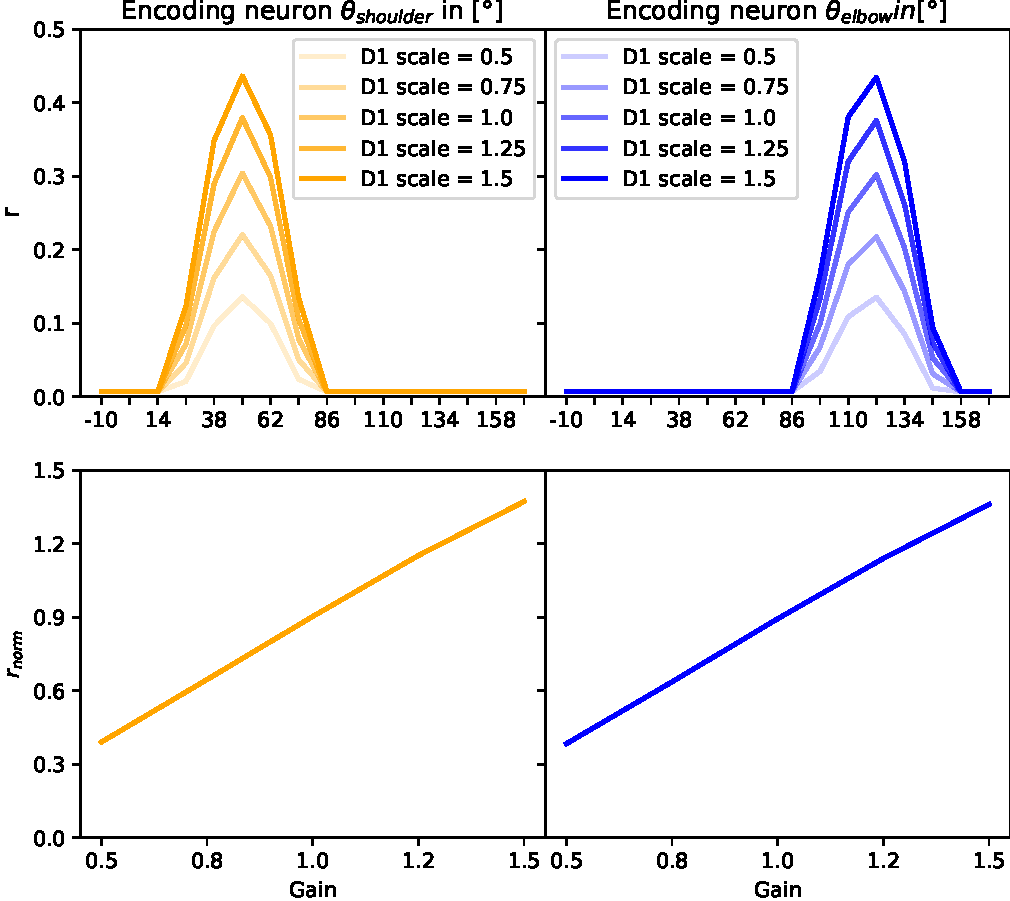
\includegraphics[width=1.1\linewidth]{d1_gain}
				\captionof{figure}{After 100 ms simulation}
			\end{center}
		\end{minipage}
		\hfill
		\begin{minipage}[t]{0.725\textwidth}
			\vspace{8pt}
			\textbf{Comparison to Deep RL:}\\[2pt]
			In order to solve the reaching task with a PPO Network \parencite{} the problem is formalised as a MDP with state $s$ and possible actions $a$:\\[5pt]
				$s = [\sin(\theta_{shoulder}, \theta_{elbow}),  \cos(\theta_{shoulder}, \theta_{elbow}), x_{error}, y_{error}]$\\
				$a = [\delta\theta_{shoulder}, \delta\theta_{elbow}]$\\[5pt]
			The reward r is defined as the negative L2 norm between current and target position (dense reward setting).
			\begin{center}
				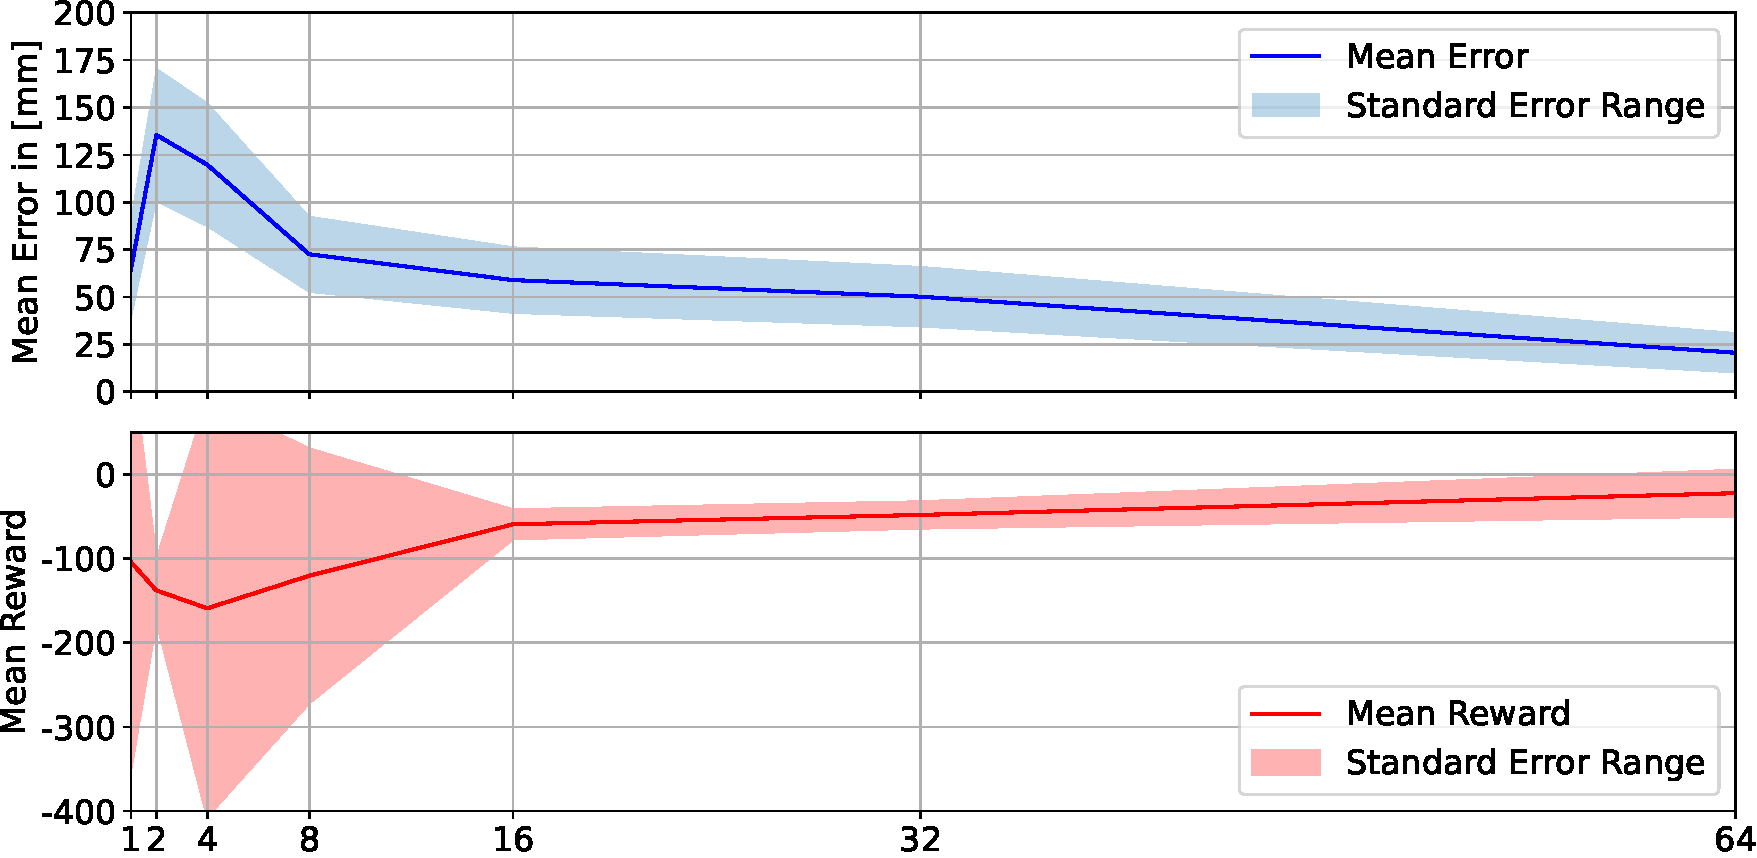
\includegraphics[width=0.8\linewidth]{ppo_error_plot}
				\captionof{figure}{Performance of the PPO trained Network}
			\end{center}
		\end{minipage}
		\hfill
	\end{adjustbox}

}


\headerbox{Training procedure}{name=res, column=0, below=model, above=refs , span=2}{
	\begin{adjustbox}{minipage=0.95\textwidth, margin=5pt, center}
		
		\begin{minipage}[t]{\textwidth}
			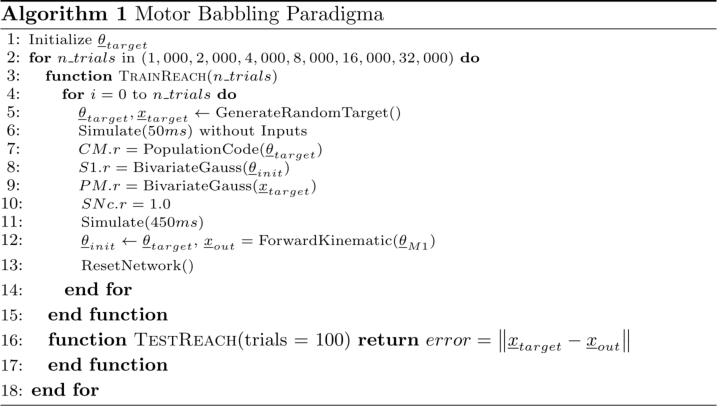
\includegraphics[width=\textwidth]{training}	
		\end{minipage}
		
	\end{adjustbox}	
}


\headerbox{\large Acknowlegdements}{name=ack, column=5, above=bottom, below=res, span=1}{	
	\begin{adjustbox}{minipage=0.925\textwidth, margin=5pt, center}
	\vfill
	This work was supported by the DFG priority program ”The Active Self” 
	HA2630/12-2.\\[2pt]
	\begin{center}
		\textit{Repository:}\\[2pt]
		
\includegraphics[width=\linewidth]{githubQR}
	\end{center}
		
	\end{adjustbox}
}


\end{poster}


\end{document}